\documentclass{beamer}
\usepackage[utf8]{inputenc}
\usepackage[T1]{fontenc}
\usepackage[francais]{babel}
\usepackage{graphicx}
\usetheme{CambridgeUS}

\title{Cloud Computing}
\author{Deng YongYan\and Barthélémy Antonin}
\institute[UM2]
{
    Université Montpellier 2
}
\date{HLIN506 TCCP, 2014}

\subject{Cloud Computing}

\pgfdeclareimage[height=1cm]{university-logo}{logo}
\logo{\pgfuseimage{university-logo}}
%
\includegraphics{logo}

\AtBeginSubsection[]
{
  \begin{frame}<beamer>{Sommaire}
    \tableofcontents[currentsection,currentsubsection]
  \end{frame}
}


\begin{document}

\begin{frame}
  \titlepage
\end{frame}

\begin{frame}{Sommaire}
  \tableofcontents
\end{frame}


\section{Origine du Cloud Computing}

\begin{frame}{Origine du Cloud Computing}
\begin{quotation}
"We didn’t care where the messages went... the cloud hid it from us."

On ne se préoccupait pas de savoir d’où venaient les messages...Le nuage en cachait l’origine.

\hfill{Kevin Marks, Google}
\end{quotation}


\end{frame}

\section{Définition pratique du Cloud Computing}


\begin{frame}{Définition pratique du Cloud Computing}
\begin{block}{Cloud Computing}
\begin{quotation}
Le Cloud Computing est un modèle Informatique qui permet un accès facile et à la demande par le réseau à un ensemble partagé de ressources informatiques configurables (serveurs, stockage, applications et services) qui peuvent être rapidement provisionnées et libérées par  un minimum d’efforts de gestion ou d’interaction avec le fournisseur du service.

\hfill{NIST (National Standard Institute)}
\end{quotation}
\end{block}
\end{frame}

\section{Les cinq caractéristiques essentielles du Cloud computing}

\begin{frame}{Les cinq caractéristiques essentielles du Cloud computing}
  \begin{itemize}
  \item {
    Accès aux services par l'utilisateur à la demande.
    \pause 
  }
  \item {   
    Accès réseau large bande.
  }
  \item<3-> {
    Réservoir de ressources (non localisées).
  }
  \item<4-> {
    Redimensionnement rapide (élasticité).
  }
  \item<5-> {
    Facturation à l'usage.
  }
  \end{itemize}
\end{frame}

\section{Les trois modèles de services}

\subsection{Software as a Service (SaaS)}
\begin{frame}{Software as a Service (SaaS)}{Logiciel en tant que service}
%\pgfdeclareimage[height=0.5cm]{service}{3service}
%\includegraphics{3service}
\begin{block}{}
\begin{quotation}
"SaaS [...] est un modèle de logiciels dans lequel ceux-ci sont installés sur des serveurs distants plutôt que sur la machine de l'utilisateur."
\hfill{Wikipedia}
\end{quotation}
\end{block}
\pause
\begin{itemize}
\item Les services de stockage en ligne.
\item Les services de visioconférence.
\item Les messageries et les logiciels collaboratifs.
\end{itemize}

\begin{figure}[centering]
    
\includegraphics[scale=0.5]{icon}
\end{figure}
\end{frame}

\subsection{Infrastructure as a Service (IaaS)}
\begin{frame}{Infrastructure as a Service (IaaS)}{Infrastructure en tant que service}
\begin{block}{}
L’utilisateur loue des moyens de calcul et de stockage, des capacités réseau et d’autres ressources indispensables (partage de charge, pare-feu, cache). 
\end{block}
\pause
\begin{block}{}
L’utilisateur ne gère pas ou ne contrôle pas l’infrastructure Cloud sous jacente mais il a le contrôle sur les systèmes d’exploitation, le stockage et les applications.
\end{block}
\pause
\begin{figure}[centering]
    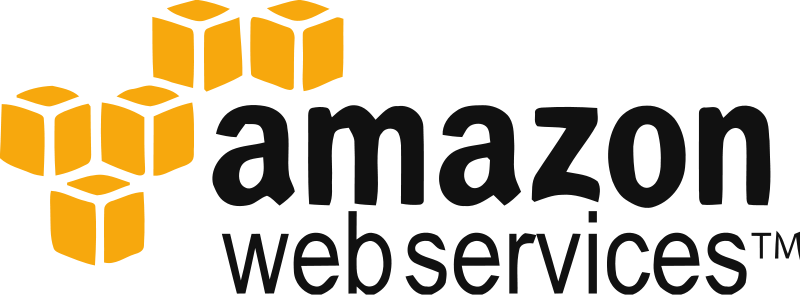
\includegraphics[scale=0.25]{amazon}
\end{figure}
\end{frame}



\subsection{Platform as a Service (PaaS)}
\begin{frame}{Platform as a Service (PaaS)}{Plate-forme en tant que service}
\begin{block}{}
L’utilisateur a la possibilité de créer et de déployer sur une PaaS ses propres applications en utilisant les langages et les outils du fournisseur.
\end{block}
\begin{block}{}
L’utilisateur ne gère pas ou ne contrôle pas l’infrastructure Cloud sous jacente (réseaux, serveurs, stockage)
\end{block}
\pause
\begin{figure}[centering]
    
\includegraphics[scale=0.4]{Paas}
\end{figure}
\end{frame}



\section{Les quatre modèles de déploiement}
\begin{frame}{Les quatre modèles de déploiement}
  \begin{block}{Cloud privé}
  L’infrastructure Cloud est utilisée par une seule organisation.
  \end{block} 
  \pause
  \begin{block}{Cloud communautaire}
  L’infrastructure Cloud est partagée par plusieurs organisations pour les besoins d’une communauté qui souhaite mettre en commun des moyens (sécurité, conformité, etc..).
  \end{block} 
  \pause
  \begin{block}{Cloud public}
  L’infrastructure cloud est ouverte au public ou à de grands groupes industriels.
  \end{block} 
  \pause
  \begin{block}{Cloud hybride}
  L’infrastructure Cloud est composée d’un ou plusieurs modèles  ci-dessus qui restent des entités séparées.
  \end{block} 
\end{frame}


\section{Les avantages du Cloud Computing}
\begin{frame}{Les avantages du Cloud Computing}
\begin{block}{Un coût inférieur}
Les clients paient uniquement l'espace de stockage qu'ils utilisent, ce qui leur permet d'économiser de l'argent.
\end{block}
\pause
\begin{block}{Une solution mobile}
Les utilisateurs peuvent accéder à leur contenu où qu'ils se trouvent, grâce à une simple connexion Internet.
\end{block}
\end{frame}

\begin{frame}{Les avantages du Cloud Computing}
\begin{block}{Une solution flexible}
Les systèmes cloud sont évolutifs : les services et l'utilisation peuvent ainsi être augmentés ou diminués à la demande, en fonction de l'activité.
\end{block}
\pause
\begin{block}{Des mises à jour logicielles automatiques}
Avec le cloud computing, la maintenance de votre serveur est réalisée par des professionnels dont c'est le métier. Leur réputation repose sur les meilleures pratiques de maintenance.
\end{block}
\end{frame}

\section{Cloud computing et sécurité}

\subsection{Avantages et défis du Cloud en terme de sécurité}
\begin{frame}{Avantages et défis du Cloud en terme de sécurité}
\begin{block}{Avantages en terme de sécurité}
  \begin{itemize}
  \item Réduit les risques pour les données internes sensibles.
  \item Rend les tests et les audits plus simples. 
  \item Permet la mise en place  de procédures automatiques accroissant notablement la sécurité.
  \end{itemize}
\end{block}
\pause
\begin{block}{Défis en terme de sécurité}
  \begin{itemize}
  \item Faut donner confiance dans le modèle de sécurité et dans les outils de gestion qui sont proposés.
  \item De manière indirecte au travers d’une interface
  \end{itemize}
\end{block}
\end{frame}


\section*{Conclusion}

\begin{frame}{Conclusion}
  \begin{itemize}
  \item
    Le Cloud computing n’est pas un effet de mode. C’est une \alert{révolution} dans la manière d’organiser, de gérer et de distribuer des ressources informatiques.
  \begin{itemize}
  \item
    « beaucoup mieux » 
  \item
    « beaucoup moins cher »
  \end{itemize}
  \end{itemize}
  
  \begin{itemize}
  \item
     Le modèle Cloud est encore très jeune et en évolution rapide.

  \end{itemize}
\end{frame}



\appendix
\section<presentation>*{\appendixname}
\subsection<presentation>*{Bibliography}

\begin{frame}[allowframebreaks]
  \frametitle<presentation>{Bibliography}
    
  \begin{thebibliography}{10}
    
  \beamertemplatearticlebibitems
  % Start with overview books.

  \bibitem{Author2012}
    Jean-Paul Figer.
    \newblock {\em L’informatique en nuage [Cloud Computing]}.
    \newblock http://www.figer.com/Publications/nuage.htm#547,  le 21 avril 2012.
 
    
  \beamertemplatearticlebibitems

  \bibitem{Someone2011}
    Raphaële Karayan.
    \newblock {\em Le cloud computing expliqué aux nuls}.
    \newblock L'Express, le 10/02/2011 à 18:23

  \beamertemplatearticlebibitems
    
  \bibitem{Someone2000}
    Raphaële Karayan.
    \newblock {\em Qu'est ce que le cloud computing: définition, avantages et intérêts}.
    \newblock http://www.salesforce.com/fr/socialsuccess/cloud-computing/Qu-est-ce-que-le-cloud-computing.jsp,2013.

  \end{thebibliography}
\end{frame}

\end{document}


